\documentclass[conference]{IEEEtran}
\IEEEoverridecommandlockouts
% The preceding line is only needed to identify funding in the first footnote. If that is unneeded, please comment it out.
\usepackage{cite}
\usepackage{amsmath,amssymb,amsfonts}
\usepackage{algorithm}
\usepackage{algpseudocode}
\usepackage{graphicx}
\usepackage{textcomp}
\usepackage{xcolor}
\usepackage{subfig}
\def\BibTeX{{\rm B\kern-.05em{\sc i\kern-.025em b}\kern-.08em
    T\kern-.1667em\lower.7ex\hbox{E}\kern-.125emX}}
\begin{document}

\title{ChimeraTL: Transfer Learning in DBMS\\with Fewer Samples\\
\thanks{NEDO and Kakenhi}
}

\makeatletter
\newcommand{\linebreakand}{%
  \end{@IEEEauthorhalign}
  \hfill\mbox{}\par
  \mbox{}\hfill\begin{@IEEEauthorhalign}
}
\makeatother

\author{\IEEEauthorblockN{Tatsuhiro Nakamori}
\IEEEauthorblockA{
    % \textit{Faculty of Media and Governance} \\
    \textit{Keio University}\\
    % Tokyo, Japan \\
    tatsuhironm@keio.jp
}
\and
\IEEEauthorblockN{Shohei Matsuura}
\IEEEauthorblockA{
    \textit{LY Corporation} \\
    % Tokyo, Japan \\
    shmatsuu@yahoo-corp.jp
}
\and
\IEEEauthorblockN{Takashi Miyazaki}
\IEEEauthorblockA{
    \textit{LY Corporation} \\
    % Tokyo, Japan \\
    takmiyaz@yahoo-corp.jp
}
\and
\IEEEauthorblockN{Sho Nakazono}
\IEEEauthorblockA{
    \textit{LY Corporation} \\
    % Tokyo, Japan \\
    shnakazo@yahoo-corp.jp
}
\linebreakand
\IEEEauthorblockN{Taiki Sato}
\IEEEauthorblockA{
    \textit{LY Corporation} \\
    % Tokyo, Japan \\
    taisato@yahoo-corp.jp
}
\and
\IEEEauthorblockN{Takashi Hoshino}
\IEEEauthorblockA{
    \textit{Cybozu Labs, Inc.} \\
    % Tokyo, Japan \\
    hoshino@labs.cybozu.co.jp
}
\and
\IEEEauthorblockN{Hideyuki Kawashima}
\IEEEauthorblockA{
    % \textit{Faculty of Environment}\\
    % \textit{and Information Studies} \\
    \textit{Keio University}\\
    % Tokyo, Japan \\
    river@sfc.keio.ac.jp
}

}

\maketitle

\begin{abstract}

\end{abstract}

\begin{IEEEkeywords}
component, formatting, style, styling, insert
\end{IEEEkeywords}

\section{Introduction}
\subsection{Motivation}\label{motivation}
Database management systems (DBMS) are an integral component of applications. One aspect of DBMS that makes it important in many applications is its adaptivity. DBMS has large amounts of configuration parameters that users can adjust in order to optimize to specific workloads and meet the user requirement. For instance, MySQL has about 190 parameters~\cite{mysql197}, while PostgreSQL offers about 170~\cite{postgre170, cdbtune}. Recent studies have put emphasis on building performance prediction models instead of relying on heuristics to find optimal configurations~\cite{iTune, Ottertune, Onlinetune, cdbtune, restune}.

While existing studies target to learn performance prediction models for unseen workloads, they assume that the model is learned from the same hardware environment as where it is used.
In reality, developers of a DBMS can test the performance of the DBMS with various configurations in a testing environment and build a performance prediction model to estimate the performance of the DBMS in the production environment\cite{Matsuura}.
Since a testing environment is often a scaled-down version of a production environment, the model learned from the testing environment may not be accurate in predicting the performance of the production environment.
What developers can do instead is to extract the knowledge of the testing environment that can be reused to build an accurate model for the production environment.

Such a model learning approach is an example of \textit{transfer learning}.
The goal of transfer learning is to reduce the learning cost (in above case, the sampling cost) in a target environment by utilizing the data from a different but related environment~\cite{l2s, datareuse}.
Studies have shown that different hardware environments exhibit similarities in the performance of DBMS, motivating the use of transfer learning techniques to exploit such similarities~\cite{Valov, jamshidi}.
% As for the developers' standpoint, by using the data from a testing environment, they can build a model with high accuracy using fewer samples from the target environment.

Our motivation is to apply transfer learning techniques to learn a DBMS performance prediction model using fewer samples from the target environment.

\subsection{Problem}
The application of transfer learning in the context of configurable software systems has been discussed\cite{l2s,Valov,jamshidi,datareuse}. 
% Each transfer learning approach takes advantage of source environment knowledge in different ways.
% For example, some studies claim that linear transformation of source model is sufficient to predict the performance in a target hardware environment as performance functions in two different environments have a linear relationship~\cite{Valov, jamshidi}.
% Another way to transfer knowledge is to include the data gathered from source environment with samples from target environment to learn the target model~\cite{datareuse}.
% There is also a systematic sampling strategy that selects the most informative samples from the target environment based on knowledge gained from source environment data.~\cite{l2s}.
While previous transfer learning approaches have been shown to be effective in certain configurable software systems, they do not consider the following DBMS parameters that must be taken into account in order to make the transfer of knowledge more effective.

\textbf{1. Parameters are not binary.}
Many of the previous studies focused their evaluation on cases in which the configuration parameters were binary, i.e., the parameter is either on or off~\cite{Valov, jamshidi, l2s}, but the parameters in DBMS often have a wide range of values.
For example, MySQL has a parameter that controls the amount of memory allocated to the buffer pool, and the value of the knob can range from 5 MB to the hardware limit~\cite{mysqlinnobuf}.
Under the assumption that source and target environments have different hardware limitations, this parameter is not even possible to be set to the same value that exceeds the limitations of the source environment.
Naively reusing the source data of such parameters would cause inaccuracies in the model, as the resulting model have no information about the performance of the parameter values that are specific to the target environment.
% Furthermore, since DBMS has numerous parameters with wide value ranges, merely sampling in a smart way is not enough to build a model effectively, as it would still require many samples to learn an accurate model for the vast configuration space.
\textbf{2. Parameters have different effects on performance in different environments.}
Although studies have shown that the performance functions of many parameters between two environments have a linear relationship~\cite{Valov, jamshidi}, employing a naive transfer learning strategy based on the assumption that all parameters follow this pattern can cause a significant bias in the model.
% Consider LineairDB\cite{lineairdb}, a database that has the number of threads as one of its parameters, for example.
Fig.~\ref{fig:valov} shows the relationship between the throughput of two environments for varying configurations in LineairDB.
From Fig.~\ref{fig:valov}, it is evident that the relationship is in fact not linear because two machines have different saturation points when the number of threads is varied.
% This example shows that some parameters are heavily machine dependent, having different effects on performance depending on the hardware limitations.

In order to build an accurate performance model of DBMS with fewer samples from the target environment, we need to take the above DBMS parameters into account by exploiting the knowledge of linear parameters while avoiding the inaccuracies caused by transferring the knowledge of non-linear parameters.
Nonetheless, to our knowledge, there is no existing transfer learning technique that considers such a design.

\subsection{Contribution}
We present ChimeraTL, a transfer learning pipeline that takes advantage of the knowledge of DBMS parameters to build an accurate performance model of DBMS with fewer samples from the target environment.
First, ChimeraTL starts by identifying two types of parameters: \textit{linear parameters} and \textit{non-linear parameters}.
Once the identification is done, ChimeraTL begins sampling the data from the target environment.
Initially, ChimeraTL focuses on collecting the data of linear parameters to learn a linear transformation between the source and target environments.
After there are enough data of linear parameters, ChimeraTL prioritizes sampling the data of non-linear parameters from the target environment.
With this strategy, ChimeraTL can reduce the number of samples while minimizing the bias caused by the difference between the source and target environments.

Central to ChimeraTL is its ability to identify which parameters are linear and which are non-linear.
Linear parameters are the ones that have similar performance effects across different environments, and non-linear parameters are the ones that have different performance effects depending on the hardware limitations as shown in Fig.~\ref{fig:valov}.
First, ChimeraTL prepares data of performance functions in two distinct environments (e.g. two docker containers with different resource restrictions in a testing environment), under the assumption that it is cheap to collect data outside the target environment. 
Then, it transforms the performance functions of a parameter to probability distributions and measure the similarity of the two distributions. 
% We use the Bhattacharyya distance~\cite{bhattacharyya} as a similarity measure in ChimeraTL as it is a symmetric measure that takes into account the difference of the whole distribution rather than the difference of mean or variance.

After the identification of the linear parameters, ChimeraTL exploits the knowledge of these parameters by applying a method that is a combination of linear transformation and data reuse.
It first samples data of the linear parameters from the target environment.
Using the sampled target data and the source data of the same parameters, ChimeraTL learns a linear transformation between the two environments.
ChimeraTL then linearly transforms the source data of linear parameters and uses them as additional training data to build a performance prediction model for the target environment.
By linearly transforming the source data, ChimeraTL can reuse the knowledge of the source environment while avoiding the bias caused by the difference between the source and target environments. 
During the above process, ChimeraTL samples the data of linear parameters more frequently than the other parameters.
However, the benefit of sampling the data of linear parameters diminishes after learning the linear transformation because the linear transformation can construct sufficient model of linear parameters in the target environment.
Once there are enough data of the linear parameters, ChimeraTL prioritizes sampling the data of non-linear parameters from the target environment.

Compared with learning the model from scratch in the target environment, ChimeraTL minimizes the prediction error to less than 10\% using 70\% fewer samples. None of the previously noted state-of-the-art transfer learning techniques\cite{l2s,Valov,datareuse} can achieve this level of accuracy with the same number of samples. 

% ChimeraTL's ability to build an accurate performance model of DBMS with fewer samples from the target environment can be applied in various scenarios.
% As mentioned in Section~\ref{motivation}, developers can use ChimeraTL to build a performance prediction model in a production environment using the data from a testing environment.
% Similarly, ChimeraTL can be used in a cloud environment where various hardware environments are available.
% Furthermore, ChimeraTL can be integrated into existing DBMS tuning systems that require pretrained models to build a performance prediction model in a new hardware environment\cite{Onlinetune,Ottertune}.
% In case the pretrained models are acquired from a different hardware environment, ChimeraTL can quickly adjust the pretrained models to the new hardware environment.
% Although ChimeraTL is designed primarily for DBMS, it can also be applied to other configurable software systems that have distinction between linear parameters and non-linear parameters.

% \subsection{Organization}
% The rest of this paper is organized as follows. 
% Section 2 revisits the transfer learning techniques used in previous studies. Section 3 describes the ChimeraTL pipeline in detail, followed by experimental evaluation in Section 4. Finally, we discuss the related work in Section 5 and conclude the paper and discuss future work in Section 6. 
\section{Preliminaries}
\label{sec:prelim}

% \subsection{Terminology}
% Here, we define the terminology used in this paper.

% 1. \textit{Configuration parameter}, or \textit{parameter} for short, is a variable that is used to configure the behavior of a software system. For example, the \texttt{client} parameter in LineairDB is used to configure the number of threads that can concurrently access the database. We use the term \textit{configuration} to denote a set of all parameters.

% 2. \textit{Environment} is a hardware setup in which a DBMS runs. 
% Source environment denotes the environment where we can readily measure the performance of a DBMS.
% Target environment is where we want to build a performance prediction model for. 
% We use the knowledge obtained from the source environment to build a model for the target environment.

% 3. \textit{Performance function} is the true relationship between the performance of a DBMS and its configuration. 
% \textit{Performance prediction model} approximates the performance function based on available data.
% $f_{env}(\boldsymbol{p_i})$ represents the performance function in an environment $env$ when a parameter is set to $\boldsymbol{p_i}$ and other parameters are set to their default values.

\subsection{Transfer Learning}
\label{sec:prelim:tl}
Transfer learning is an active research area that aims to reduce the cost of building a model by utilizing the knowledge obtained from a different but related source.
In this paper, we compare with the transfer learning techniques that have been proposed for the performance prediction of configurable software systems.

1. \textit{ModelShift} is a type of transfer learning where the performance model learned from the source environment is linearly transformed to predict the performance of the target environment\cite{Valov}. Essentially, this method constructs a linear regression model that reflects the relationship between the performance of the source and target environments, as in Fig.~\ref{fig:valov}. Previous study has shown that ModelShift requires less than 10 samples from the target environment to learn the linear regression model\cite{Valov}. 

2. \textit{DataReuseTL} is an approach to use the source environment data in addition to data samples from the target environment to build a performance prediction model\cite{datareuse}. 
DataReuseTL works especially well even with few samples from the target environment when the source and target environments have small differences.

3. \textit{L2S} extracts information that are likely to be shared between the source and target environments\cite{jamshidi}, and uses them to build a model for the target environment\cite{l2s}.
Because this method does not use the source environment data for model construction, there are no concerns about the bias caused by the difference between the source and target environments.

\subsection{Limitations of Existing Transfer Learning Methods}
\label{sec:prelim:limitation}

\begin{figure*}[htbp]
  \centering
  \begin{minipage}{.4\textwidth}
    \centering
    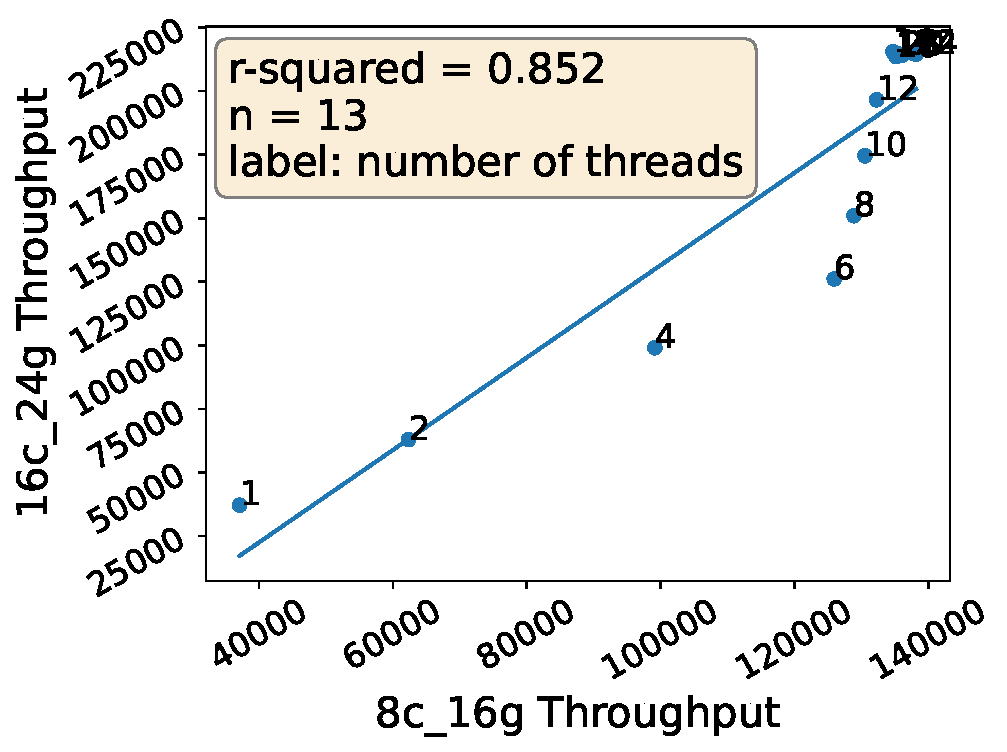
\includegraphics[width=.7\linewidth]{src/fig/rw8_vs_16.pdf}
    \caption{\textbf{Relationship of LineairDB\cite{lineairdb} throughput between two environments and a linear regression model} -- The label on each point shows the value of the parameter. The x-axis represents the throughput of 8 core 16 GB memory machine while the y-axis represents the throughput of 16 core 24 GB memory machine.}
    \label{fig:valov}
  \end{minipage}%
  \hfill
  \begin{minipage}{.55\textwidth}
    \centering
    \subfloat[Linear parameter]{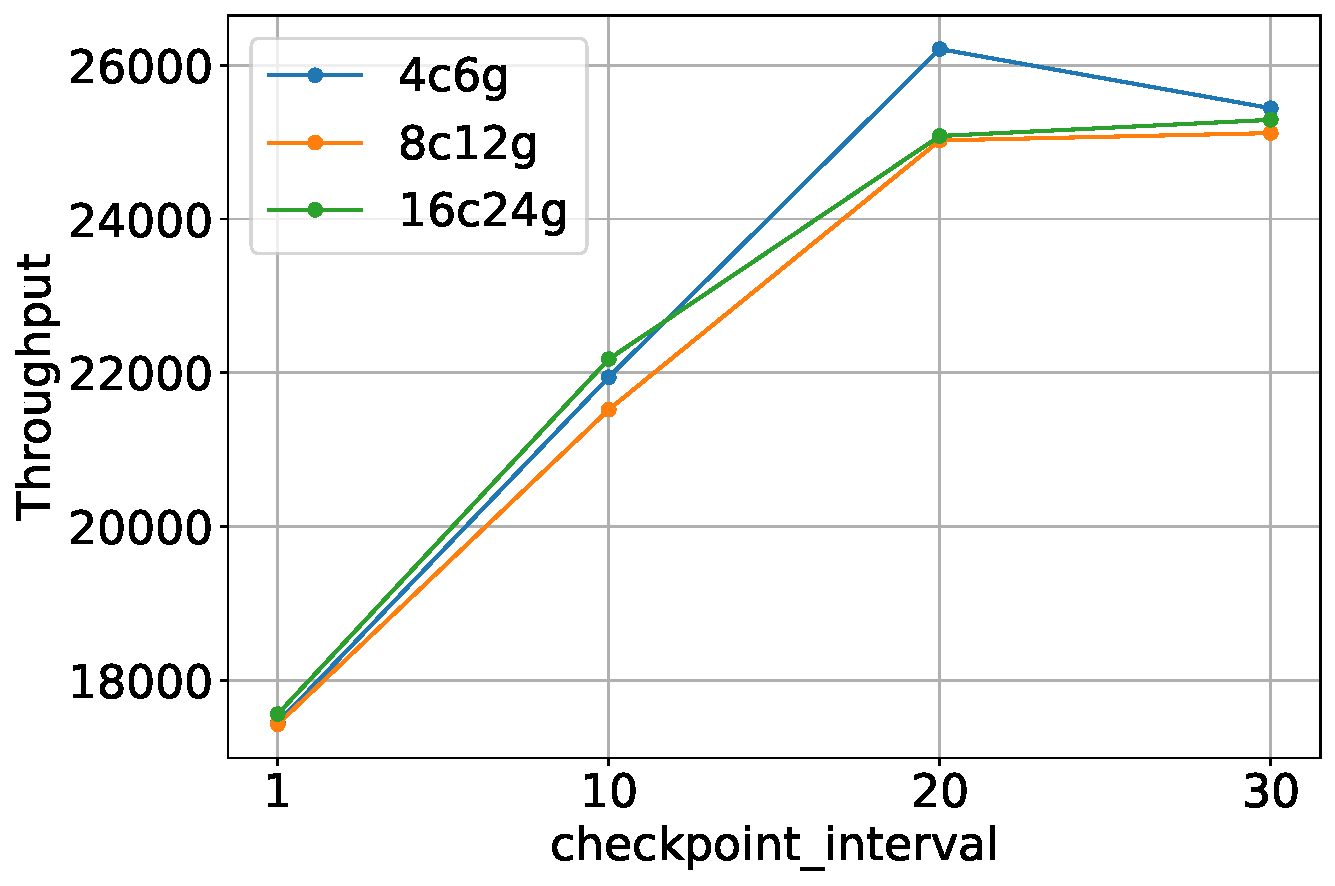
\includegraphics[width=.45\linewidth]{src/fig/checkpoint_interval.pdf}\label{fig:param:related}}
    \hfill
    \subfloat[Non-linear parameter]{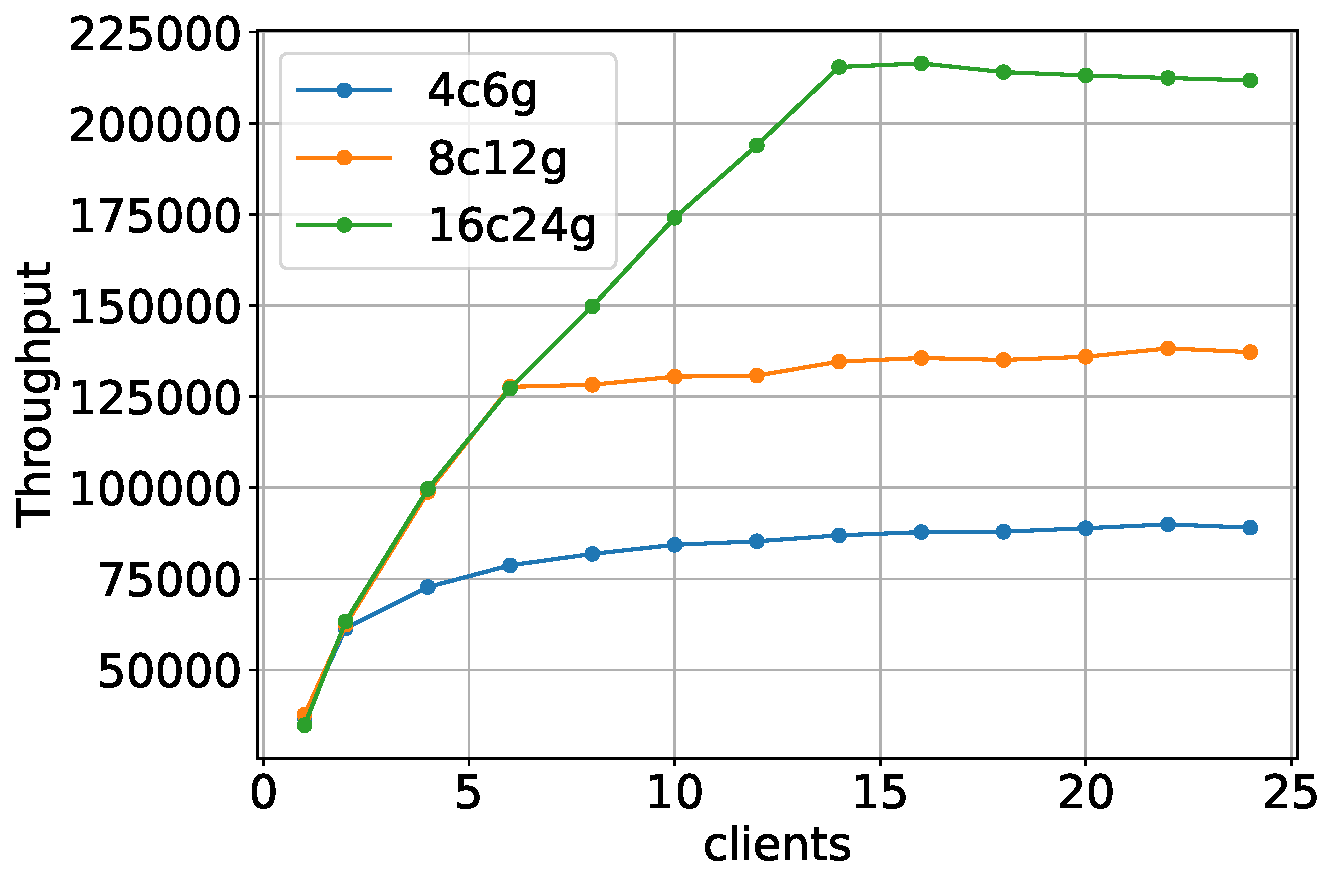
\includegraphics[width=.45\linewidth]{src/fig/clients.pdf}\label{fig:param:independent}}
    \caption{\textbf{Performance functions of linear and non-linear parameters} -- Each line represents the performance function of a parameter in a different environment. For example, 4c6g represents the performance function of a parameter in an environment with 4 CPU cores and 6 GB of memory.}
    \label{fig:params}
  \end{minipage}
\end{figure*}

Parameters in DBMS (and other configurable software systems) can be categorized into two types: \textit{linear} and \textit{non-linear}.

Linear parameters are the parameters that affect the performance of a DBMS similarly in different environments.
Formally, a parameter $\boldsymbol{p_i}$ is linear if it satisfies the following equation:
\begin{equation}
    f_{tgt}(\boldsymbol{p_i}) = \beta{\times}f_{src}(\boldsymbol{p_i})+\beta_0\label{linear}
\end{equation}
where $f_{tgt}(\boldsymbol{p_i})$ represents the performance function in a target environment, and $\beta{\times}f_{src}(\boldsymbol{p_i})+\beta_0$ denotes a linear transformation of the performance function in a source environment.
Fig.~\ref{fig:param:related} shows an example of a linear parameter in LineairDB.
The figure shows that the performance function of the parameter have similar shapes in different environments, and that the performance in one environment can be approximated by linearly transforming the performance in another environment.
This result suggests that source environment data of linear parameters can be readily reused after an appropriate linear transformation to build a model for the target environment.
Considering that it takes less than 10 samples from the target environment to learn the linear transformation\cite{Valov}, the data of linear parameters from the source environment should be exploited in order to build a model using fewer samples from the target environment.

The remaining parameters are non-linear parameters that behave differently in different environments.
Fig.~\ref{fig:param:independent} shows an example of a non-linear parameter.
The three different environments in the figure have different performance trends for the same parameter value due to the difference in saturation points.
In the context of transfer learning, using the data of non-linear parameters from the source environment to build a model for the target environment is problematic because the data from the source environment may not reflect the true relationship between the performance and the parameter values in the target environment.
As a result, the source data would negatively interfere with the learning of the performance function in the target environment (i.e. negative transfer), and the accuracy of the model would be degraded.
In order to avoid the negative transfer, the source environment data of non-linear parameters should be excluded from the model construction.

Each of the transfer learning methods described in Section~\ref{sec:prelim:tl} does not consider the difference between linear and non-linear parameters, which leads to disadvantages in different ways.
ModelShift and DataReuseTL work well under the assumption that all parameters are linear, but since non-linear parameters in DBMS may have varying effects on the performance depending on the underlying hardware environment, the resulting model may suffer from a bias caused by the difference between the source and target environments.
% the accuracy of the resulting model is constrained by the extent to which these parameters do not significantly influence performance.
Similarly, L2S does not distinguish between non-linear and linear parameters.
Because L2S does not use the source environment data for model construction, there are no concerns about the negative transfer caused by the difference between the source and target environments.
However, it does not exploit the source environment data of linear parameters, losing on the opportunity to reduce the amount of samples necessary from the target environment to build a practical model.
This is especially problematic in the case of DBMS. 
Since the parameter space of DBMS is vast, L2S has to compensate for the lack of source environment data by collecting more samples from the target environment.
We need to differentiate between linear and non-linear parameters in order to build a DBMS performance prediction model with high accuracy using fewer samples from the target environment.
\section{ChimeraTL}
% \subsection{Overview}
ChimeraTL is a novel transfer learning method that combines the elements of ModelShift, DataReuseTL, and L2S in a way that maximizes their advantages and minimizes their disadvantages.
It consists of three procedures: (1) parameter selection and separation, (2) linear transformation learning, and (3) non-linear parameter learning.

\subsection{Parameter Selection and Separation}
\label{sec:parameter_selection}
The first step of ChimeraTL is to select parameters that have a significant impact on performance and separate them into linear parameters and non-linear parameters.

In the studies of DBMS performance models, parameter selection is a common practice because the number of parameters in DBMS is usually large, and not all of them have a significant impact on performance\cite{mysql197,Ottertune}.
Parameter selection can be done manually by experts, but it is time-consuming and requires a deep understanding of the DBMS.
Therefore, we use a feature selection method that automatically selects parameters that have a significant impact on performance.
As in L2S\cite{l2s}, we use stepwise regression\cite{stepwise} as the feature selection method.

While many studies have incorporated parameter selection into their approach, to the best of our knowledge, there is no existing method that separates parameters into linear and non-linear parameters.
Therefore, we propose a novel algorithm that uses Bhattacharyya distance\cite{bhattacharyya} to separate parameters based on the difference in their performance functions between two environments.

% TODO: make the algorithm more correct
\begin{algorithm}\small
  \caption{Parameter separation}
  \label{alg:separation}
  \begin{algorithmic}[1]
      \Require 
        \Statex $\boldsymbol{P}$: set of parameters
        \Statex $f_{1}$: performance function in environment 1
        \Statex $f_{2}$: performance function in environment 2
        \Statex $T$: threshold
      \Ensure 
        \Statex $\boldsymbol{P_{lr}}$: set of linear parameters
        \Statex $\boldsymbol{P_{nl}}$: set of non-linear parameters
      \Statex

      \State $\boldsymbol{P_{lr}} \gets \emptyset$
      \State $\boldsymbol{P_{nl}} \gets \emptyset$
      \For{$\boldsymbol{p_i} \in \boldsymbol{P}$}
          \State $p_{1}(\boldsymbol{p_i}) \gets \text{normalize}(f_{1}(\boldsymbol{p_i}))$\label{alg:separation:norm1}
          \State $p_{2}(\boldsymbol{p_i}) \gets \text{normalize}(f_{2}(\boldsymbol{p_i}))$\label{alg:separation:norm2}
          \State $d \gets \text{BhattacharyyaDistance}(p_{1}(\boldsymbol{p_i}), p_{2}(\boldsymbol{p_i}))$\label{alg:separation:distance}
          \If{$d < T$}\label{alg:separation:threshold}
              \State $\boldsymbol{P_{lr}} \gets \boldsymbol{P_{lr}} \cup \boldsymbol{p_i}$
          \Else
              \State $\boldsymbol{P_{nl}} \gets \boldsymbol{P_{nl}} \cup \boldsymbol{p_i}$
          \EndIf
      \EndFor
      \State \Return $\boldsymbol{P_{lr}}$, $\boldsymbol{P_{nl}}$
  \end{algorithmic}
\end{algorithm}

Bhattacharyya distance is a measure of the similarity between two probability distributions.
There are two advantages of using Bhattacharyya distance for parameter separation.
First, Bhattacharyya distance takes into account the shape of the probability distributions.
As opposed to only comparing the mean, variance, or largest absolute difference between two distributions\cite{kstest}, Bhattacharyya distance considers the entire distribution.
Even if two distributions have similar trends for some values, Bhattacharyya distance will be large if they have different trends for other values.
Second, Bhattacharyya distance is a symmetric measure, meaning that the distance between two distributions is the same regardless of which distribution is used as the reference.
Because of this property, setting a threshold on the distance is intuitive and easy to interpret.

The parameter separation algorithm is shown in Algorithm~\ref{alg:separation}.
The initial step of the algorithm is to convert each performance function of a parameter into a probability distribution.
This is done by normalizing the performance function so that the sum of the measured values becomes 1 (Line \ref{alg:separation:norm1}, \ref{alg:separation:norm2}).
Then, the Bhattacharyya distance between the two probability distributions is calculated (Line \ref{alg:separation:distance}).
If the distance is smaller than a threshold $T$, the parameter is considered to be linear, and otherwise it is considered to be non-linear (Line \ref{alg:separation:threshold}).
ChimeraTL uses the threshold to decide the trade-off between including more parameters in the linear group to reduce the number of samples required for model construction, and including more parameters in the non-linear group to reduce the risk of negative transfer.
The intuition behind this algorithm is that the parameters that have a performance function with a similar shape in different environments are likely to be linear, and vice versa (Fig.~\ref{fig:params}).


\subsection{Sampling in the Target Environment}
Once the parameters are separated into linear and non-linear parameters, ChimeraTL is ready to collect data from the target environment. 
There are two ways ChimeraTL collects data from the target environment.
For the first few samples, ChimeraTL focuses on collecting data of linear parameters to learn the linear transformation between the source and target environments.
With just a few samples, ChimeraTL can learn the linear transformation and reuse the source environment data of linear parameters for target model construction.
After collecting a set amount of samples for linear transformation learning, ChimeraTL prioritizes collecting data of non-linear parameters which are not available in the source environment.

One iteration of the sampling process is shown in Algorithm~\ref{alg:sampling}.
The sampling rate of linear parameters ($lr$) and the number of samples for priority switching ($N$) are the two parameters of ChimeraTL that control the sampling process.
In our implementation, we set $lr$ to 90\% initially, and switch to 10\% after collecting 5 samples for linear transformation learning (Line \ref{alg:sampling:n}, \ref{alg:sampling:lr}).

At the end of each iteration, ChimeraTL fits a performance prediction model using the collected data.
We use Gaussian Process (GP) regression\cite{gp} as the performance prediction model because it is known to be effective in modeling the performance of configurable software systems\cite{l2s,Ottertune,restune,Onlinetune,datareuse}.

\begin{algorithm}\small
  \caption{Sampling in the target environment}
  \label{alg:sampling}
  \begin{algorithmic}[1]
    \Require
      \Statex $\boldsymbol{P_{lr}}$: set of linear parameters
      \Statex $\boldsymbol{P_{nl}}$: set of non-linear parameters
      \Statex $N$: number of samples for priority switching
      \Statex $lr$: sampling rate of linear parameters
      \Statex $f_{src}$: performance function in the source environment
      \Statex $\text{model}$: performance prediction model
    \Ensure 
      \Statex $D_{tgt}$: target data
      \Statex $D_{lr}^{tgt}$: target data of linear parameters
      \Statex $D_{lr}^{src}$: source data of linear parameters
    \Statex

    \Function{RunNextIteration}{}
      \State $\text{sample\_linear} \gets \text{Random}() < lr$
      \If{$\text{sample\_linear}$}
        \State $\text{SampleLinear}()$
        \If{$\text{size}(D_{lr}^{tgt}) = N$}\label{alg:sampling:n}
          \State $lr \gets 1 - lr$\label{alg:sampling:lr}
        \EndIf
      \Else
        \State $\text{SampleNonLinear}()$
      \EndIf
      \State $\text{FitModel}(D_{train})$
    \EndFunction

    \State

    \Function{SampleLinear}{}\label{alg:sampling:regression}
      \State $\boldsymbol{p_i} \gets \text{RandomChoice}(\boldsymbol{P_{lr}})$
      \State $D_{lr}^{src} \gets D_{lr}^{src} \cup \{f_{src}(\boldsymbol{p_i}\}$
      \State $D_{lr}^{tgt} \gets D_{lr}^{tgt} \cup \{\text{sample}(f_{tgt}(\boldsymbol{p_i})\}$
      \State $\text{regression\_data} \gets \text{MergeOnConfig}(D_{lr}^{src}, D_{lr}^{tgt})$
      \State $\boldsymbol{\beta} \gets \text{LinearRegression}(\text{regression\_data})$
      \State $D_{tgt} \gets D_{tgt} \cup \{f_{tgt}(\boldsymbol{p_i})\}$
    \EndFunction

    \State

    \Function{SampleNonLinear}{}
      \State $\boldsymbol{p_i} \gets \text{RandomChoice}(\boldsymbol{P_{nl}})$
      \State $D_{tgt} \gets D_{tgt} \cup \{f_{tgt}(\boldsymbol{p_i})\}$
    \EndFunction

    \State

    \Function{FitModel}{}
      \State $\text{linearly\_related\_data} \gets \{f_{src}(\boldsymbol{p_i}) \,|\, \boldsymbol{p_i} \in \boldsymbol{P_{lr}}\}$
      \State $\text{data} \gets \text{Transform}(\text{linearly\_related\_data}, \boldsymbol{\beta})$\label{alg:sampling:transform}
      \State $\text{data} \gets \{d \in \text{data} \,|\, \text{Config}(d) \notin \text{Config}(D_{tgt})\}$
      \State $\text{data} \gets \text{data} \cup D_{tgt}$\label{alg:sampling:alldata}
      \State $\text{model.fit}(\text{data})$
    \EndFunction
    
  \end{algorithmic}
\end{algorithm}

\subsubsection{Linear Transformation Learning}
Learning the linear transformation between the source and target environments is an essential step that enables ChimeraTL to reuse the data of linear parameters from the source environment.
Reusing the linearly transformed source data dramatically reduces the number of samples from the target environment required to build a model.

Each time a new sample of linear parameters is collected from the target environment, ChimeraTL merges the sample with the source environment data of the same configuration and fits a linear regression model to the merged data (Line \ref{alg:sampling:regression}).
The linear regression model is used to transform the data of linear parameters in the source environment into an estimation of the data in the target environment (Line \ref{alg:sampling:transform}).
The transformed data is then combined with the samples from the target environment to build a performance prediction model (Line \ref{alg:sampling:alldata}).

Unlike ModelShift\cite{Valov}, ChimeraTL does not assume that all the parameters are linear.
Constructing a linear regression model using all the parameters would cause negative transfer because the non-linear parameters may not follow the pattern of the linear parameters.
Instead, ChimeraTL only samples the data of linear parameters selected in Section~\ref{sec:parameter_selection} to learn the linear regression.
Similarly, the linear regression model is only used to transform the source data of linear parameters, and the source data of non-linear parameters are not used in the target model construction.

\subsubsection{Non-linear Parameter Learning}
Initially, ChimeraTL samples the data of linear parameters more frequently than the other parameters.
However, the benefit of sampling those data diminishes after learning the linear transformation because the linearly transformed source data can substitute the target environment data of linear parameters for model construction.
Once there are enough data of the linear parameters, ChimeraTL prioritizes sampling the data of non-linear parameters from the target environment.
This strategy is based on the fact that the non-linear parameters have different effects on performance depending on the hardware limitations, and the trends of these parameters are not observable in the source environment.
Therefore, ChimeraTL collects the data of non-linear parameters more often than the other parameters to learn the target-environment specific trends of these parameters.

% TODO: write about GP
\section{Evaluation}
\label{sec:eval}

We evaluate the performance of ChimeraTL in terms of the accuracy of the performance prediction model it builds.
We compare ChimeraTL with the following four methods: \textit{ModelShift}, \textit{DataReuseTL}, \textit{L2S}, and \textit{L2S+DataReuseTL} (a combined approach of DataReuseTL and L2S\cite{l2s}). 

Although original papers of ModelShift and DataReuseTL do not conduct parameter selection, we perform parameter selection using stepwise regression\cite{stepwise} for these methods to achieve the best performance.
In addition, we use the same Gaussian Process regression model as the performance prediction model for all the methods to ensure a fair comparison of transfer learning approaches.

\subsection{Experimental Setup}
\label{sec:eval:setup}
For all the experiments, we use LineairDB\cite{lineairdb} to generate performance data.
LineairDB~\cite{lineairdb} is an open-source transactional key-value storage engine based on Silo~\cite{silo}.
% LineairDB incorporates NWR~\cite{nakazono} in its implementation of optimistic concurrency control. 
% In addition, it provides efficient logging by epoch-based group commit. 
% Both of these factors support LineairDB's high performance and scalability for various workloads in many-core environments.
The parameter space of LineairDB considered in this paper is shown in Table~\ref{tab:lineairdb}.
\begin{table}[t]
    \caption{Parameter space of LineairDB}
    \label{tab:lineairdb}
    \centering
    \begin{tabular}{|c|c|c|}
        \hline
        \textbf{Parameter} & \textbf{Range} & \textbf{Default value} \\
        \hline
        \texttt{clients} & 1-24 & 1 \\
        \hline
        \texttt{checkpoint\_interval} & 1-30 & 30 \\
        \hline
        \texttt{epoch\_duration} & 1-40 & 40 \\
        \hline
        \texttt{prefetch\_locality} & 0-3 & 3 \\
        \hline
        \texttt{rehash\_threshold} & 0.1-0.99 & 0.8 \\
        \hline
    \end{tabular}
\end{table}

Table \ref{tab:env} shows the source and target environments used in the experiments.
For the source environment, we set up a docker container on a MacBook Pro with Apple M3 Max processor (16 cores) and 48 GB memory.
Conversely, we use a server with Intel(R) Xeon(R) Gold 6130 CPU (2.10GHz, 64 cores) and 1.6 TB memory to host a docker container for the target environment.
Docker containers are used to restrict the amount of resources available to each environment.
We use two completely different host machines to simulate the case where developers test their software on a local machine and deploy it on a server.

\begin{table}[tb]
    \caption{Source and target environments}
    \label{tab:env}
    \centering
    \begin{tabular}{|c|c|c|}
        \hline
        \textbf{Environment} & \textbf{Source} & \textbf{Target} \\
        \hline
        \textbf{\#Cores} & 8 & 24 \\
        \hline
        \textbf{RAM size} & 12 GB & 32 GB \\
        \hline
        \textbf{Host Machine CPU} & Apple M3 Max &  Intel(R) Xeon(R) Gold 6130 \\
        & (16 cores) & (64 cores) \\
        \hline
        \textbf{Host Machine RAM size} & 48GB & 1.6TB \\
        \hline
    \end{tabular}
\end{table}

We measure the performance of LineairDB by running the Yahoo! Cloud Serving Benchmark (YCSB)\cite{ycsb} with the workload A.
In all the experiments, we assume that the workload is the same between the source and target environments.
This assumption is realistic because application developers test their software for expected workloads before deploying it to the target environment.
For the performance metric, we use the throughput of the database, which is the number of transactions processed per second.

% Since the goal of this paper is to propose a transfer learning method that can build an accurate performance prediction model with fewer samples from the target environment, we evaluate each transfer learning method in terms of the number of samples required to build a model with a certain accuracy.
% As the accuracy metric, we use mean absolute percentage error (MAPE), which is defined as follows:
% \begin{equation}
%     \label{eq:mape}
%     \text{MAPE} = \frac{1}{n}\sum_{i=1}^{n}\left|\frac{y_i - \hat{y}_i}{y_i}\right|
% \end{equation}
% where $y_i$ is the actual performance of the $i$-th sample, $\hat{y}_i$ is the predicted performance of the $i$-th sample, and $n$ is the number of samples.
% MAPE is a common scale-independent metric for evaluating the accuracy of performance prediction models\cite{Valov, l2s, mape}.
% We run each experiment 5 times and calculate the average MAPE.

\subsection{Comparison with Existing Methods}
\label{sec:eval:exst}
% \begin{figure*}[th]
%     \centering 
%     \begin{minipage}{.325\textwidth}
%         \centering
%         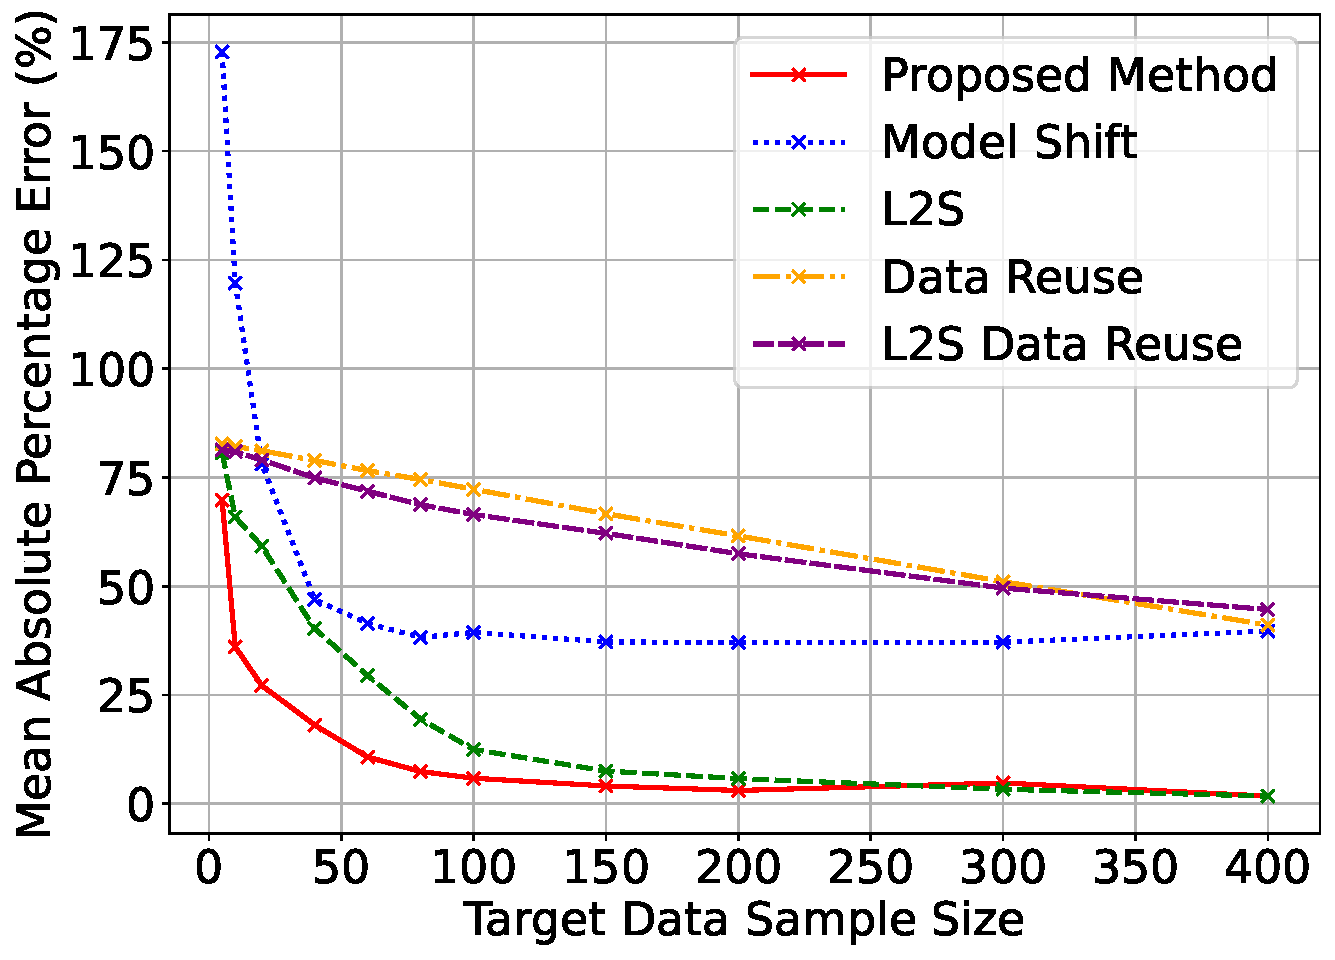
\includegraphics[width=.9\linewidth]{src/fig/tl.pdf}
%         \caption{\textbf{Performance prediction accuracy of transfer learning methods}}
%         \label{fig:results}
%     \end{minipage}
%     \hfill
%     \begin{minipage}{.325\textwidth}
%         \centering
%         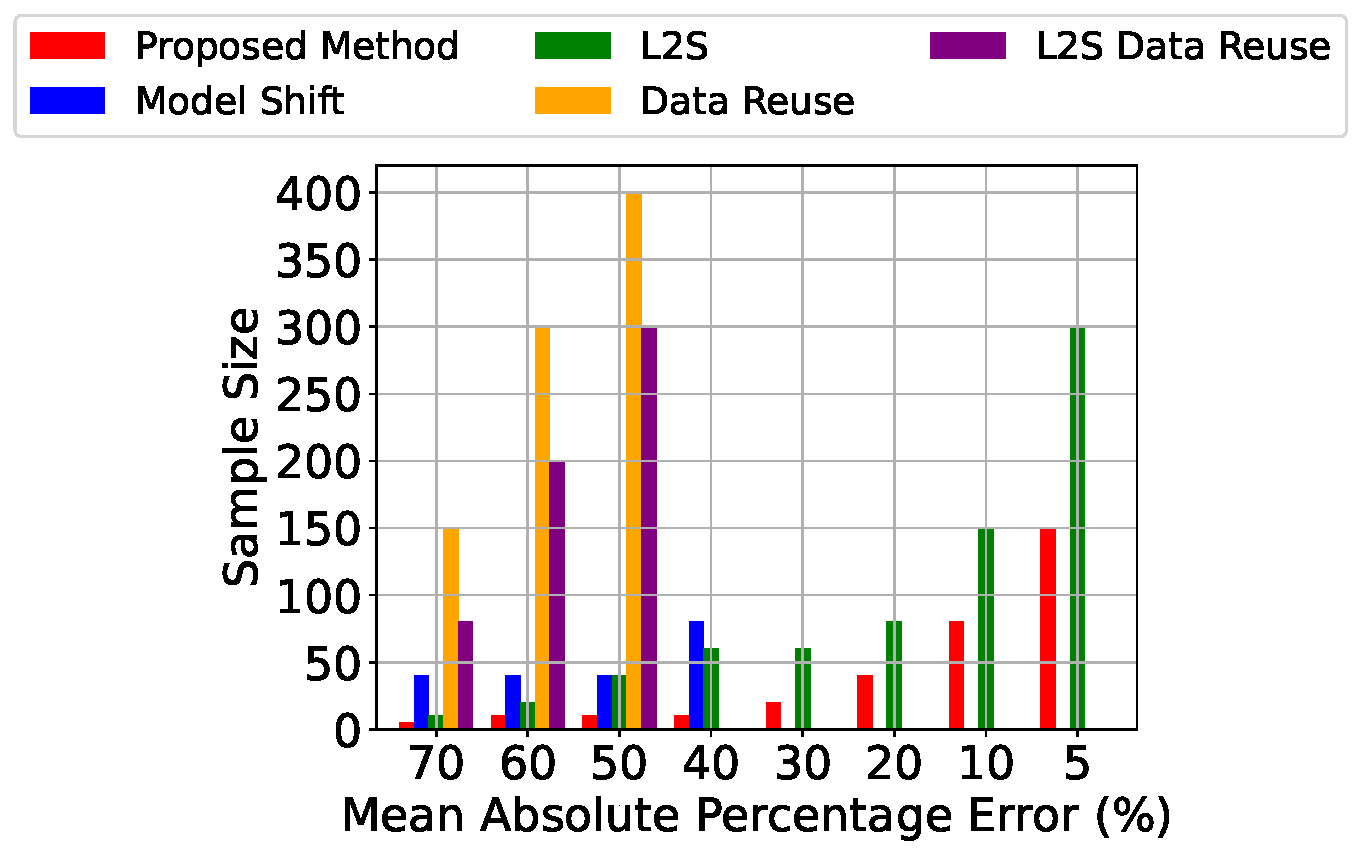
\includegraphics[width=1\linewidth]{src/fig/tl_bar.pdf}
%         \caption{\textbf{Minimum samples required for improved prediction accuracy} -- ModelShift, DataReuseTL, and L2S+DataReuseTL cannot reduce the error below 40\% even with all the samples from the target environment.}
%         \label{fig:bar}
%     \end{minipage}
%     \hfill
%     \begin{minipage}{.325\textwidth}
%         \centering
%         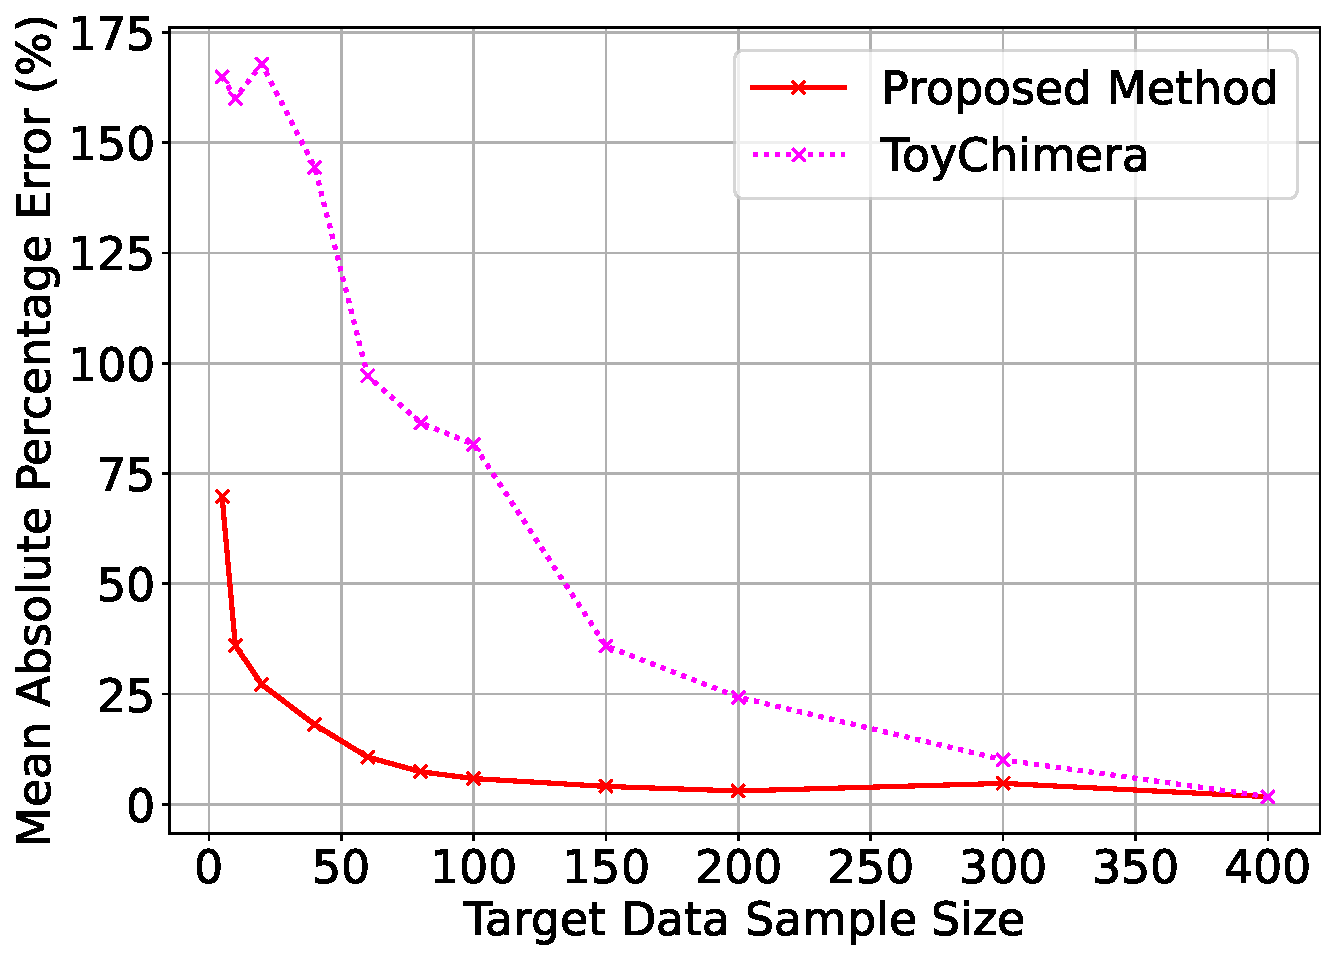
\includegraphics[width=.9\linewidth]{src/fig/toy.pdf}
%         \caption{\textbf{Performance prediction accuracy of ChimeraTL and ToyChimera}}
%         \label{fig:toy}
%     \end{minipage}
% \end{figure*}
% \begin{figure*}[th]
%     \centering
%     \begin{minipage}{.45\textwidth}
%         \centering
%         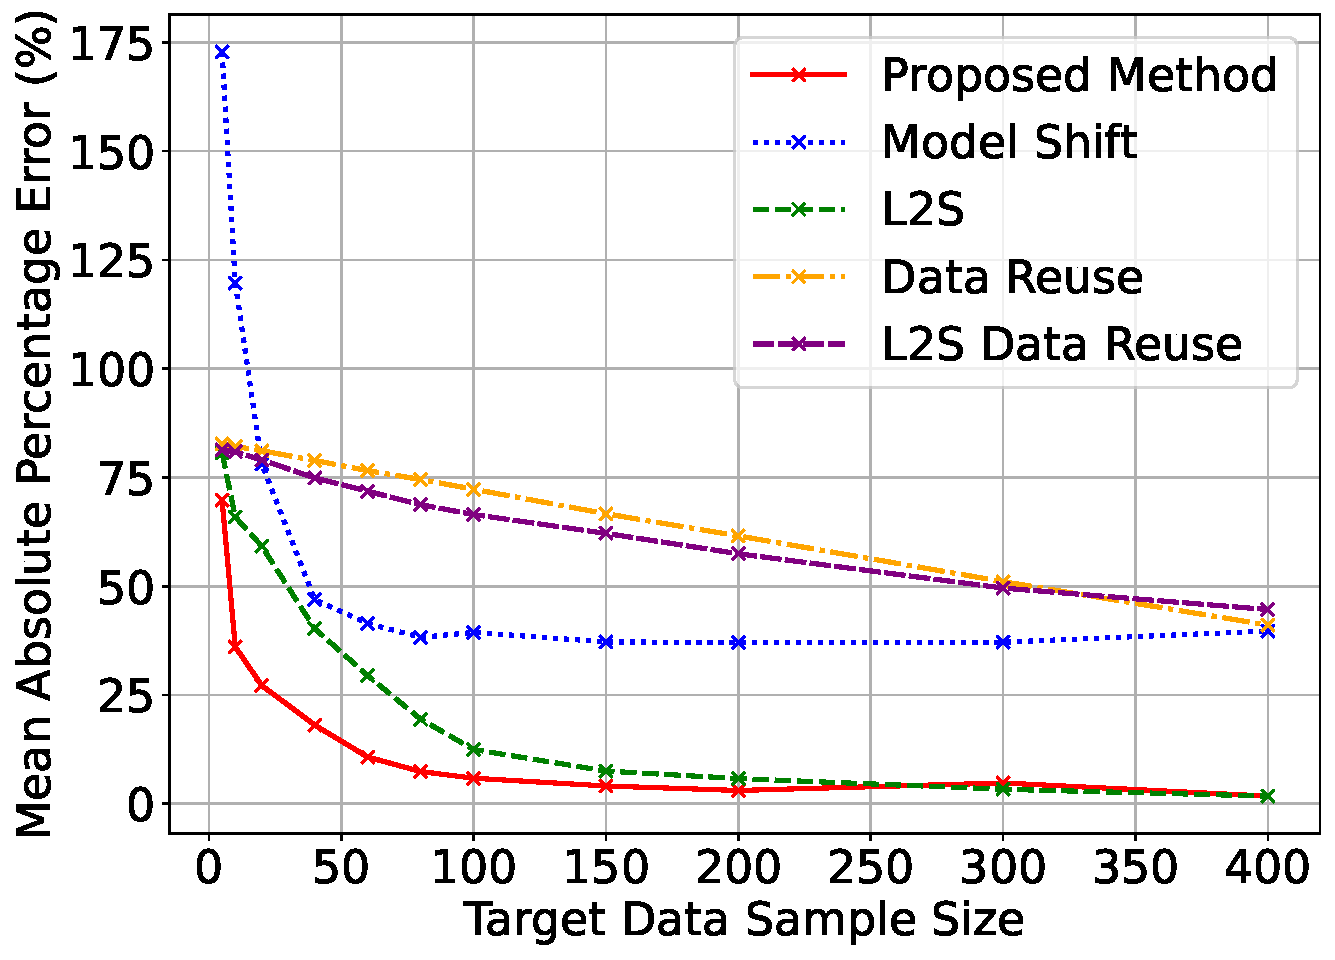
\includegraphics[width=.7\linewidth]{src/fig/tl.pdf}
%         \caption{\textbf{Performance prediction accuracy of transfer learning methods}}
%         \label{fig:results}
%     \end{minipage}%
%     \hfill
%     \begin{minipage}{.45\textwidth}
%         \centering
%         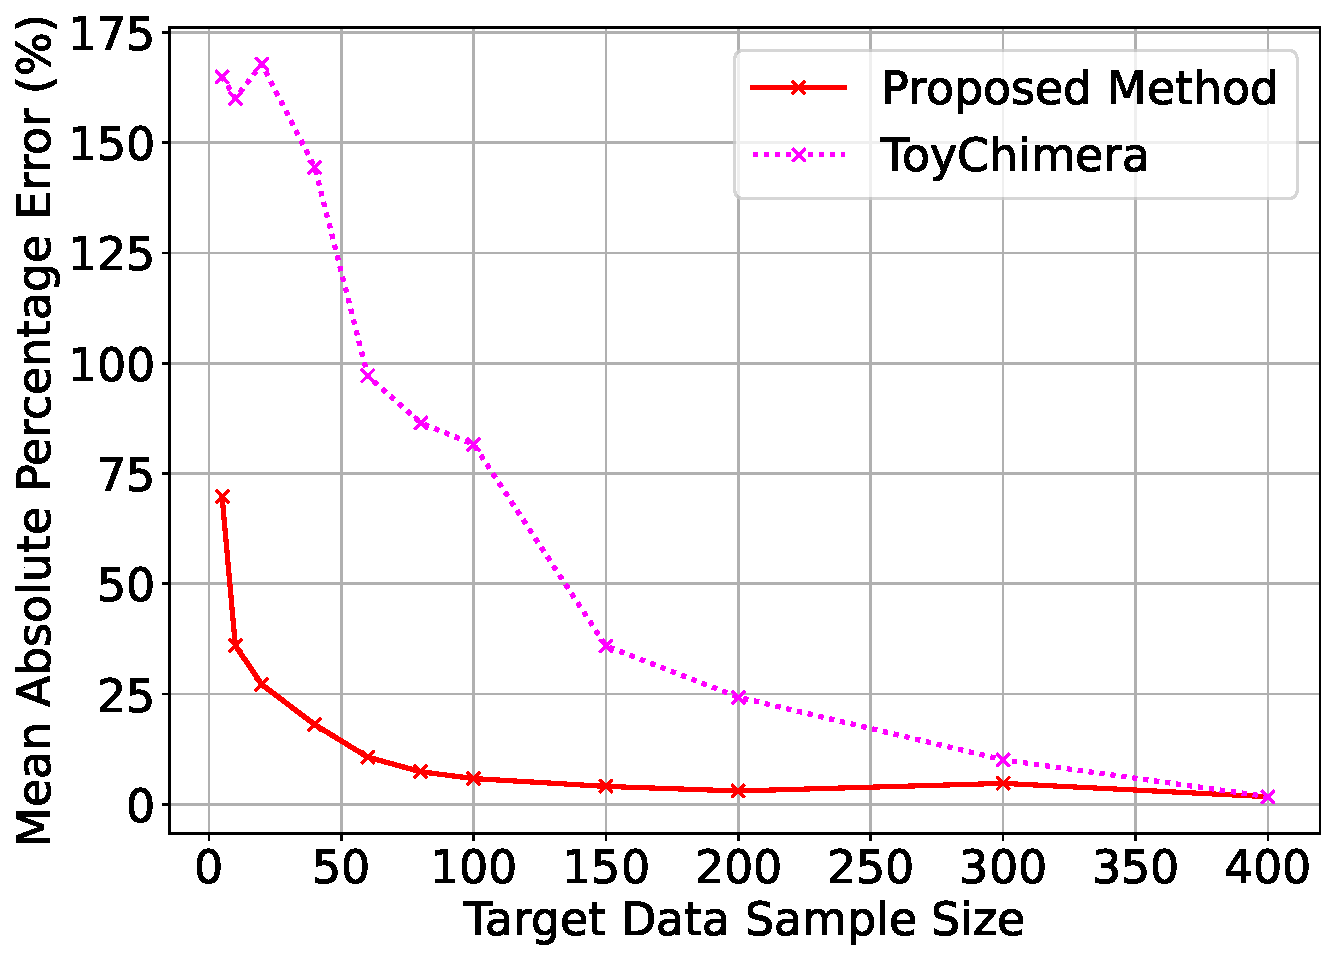
\includegraphics[width=.7\linewidth]{src/fig/toy.pdf}
%         \caption{\textbf{Performance prediction accuracy of ChimeraTL and ToyChimera}}
%         \label{fig:toy}
%     \end{minipage}
% \end{figure*}
\begin{figure*}[th]
    \centering
    \begin{minipage}{.45\textwidth}
        \centering
        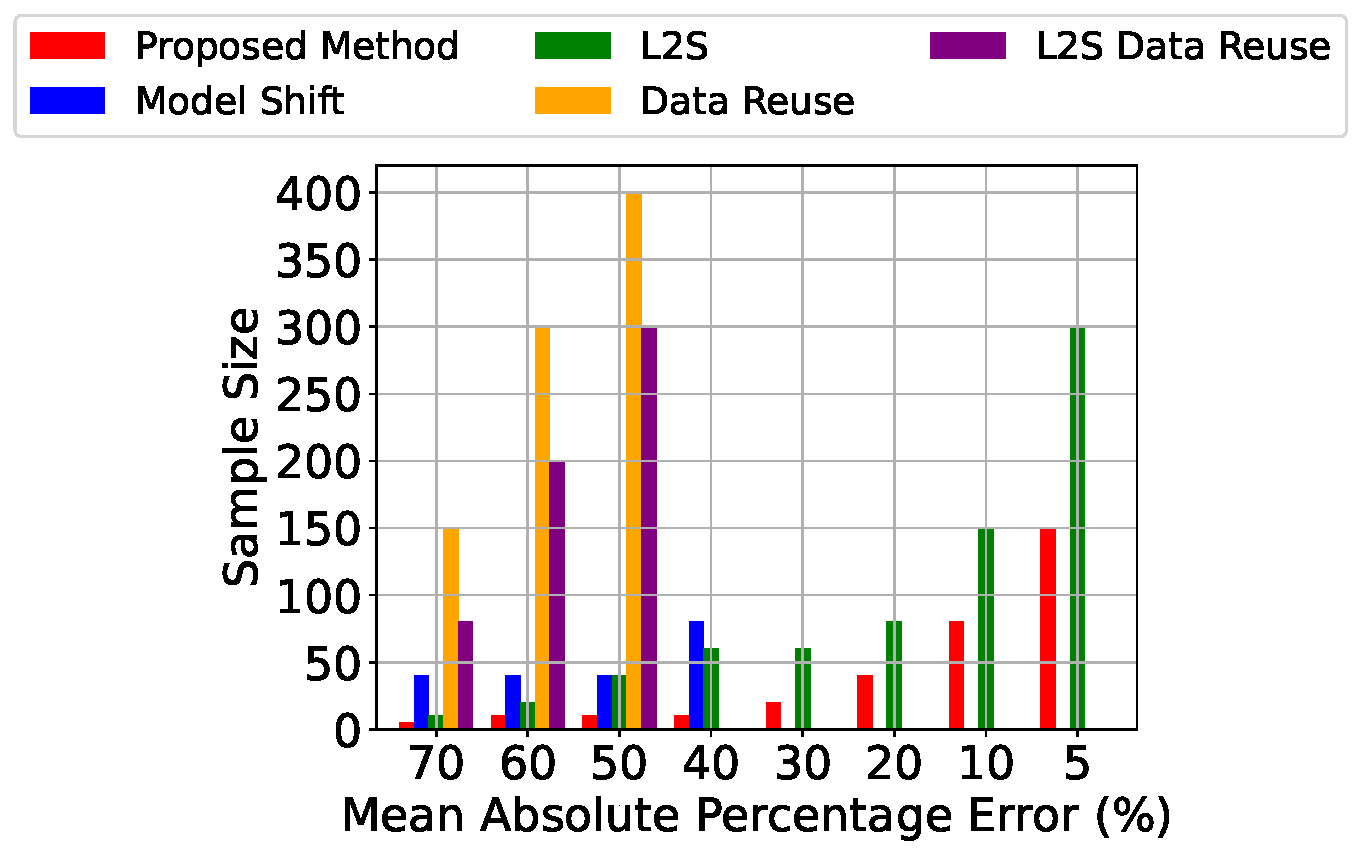
\includegraphics[width=1\linewidth]{src/fig/tl_bar.pdf}
        \caption{\textbf{Performance prediction accuracy of transfer learning methods} -- ModelShift, DataReuseTL, and L2S+DataReuseTL cannot reduce the error below 40\% even with all the samples from the target environment.}
        \label{fig:results}
    \end{minipage}%
    \hfill
    \begin{minipage}{.45\textwidth}
        \centering
        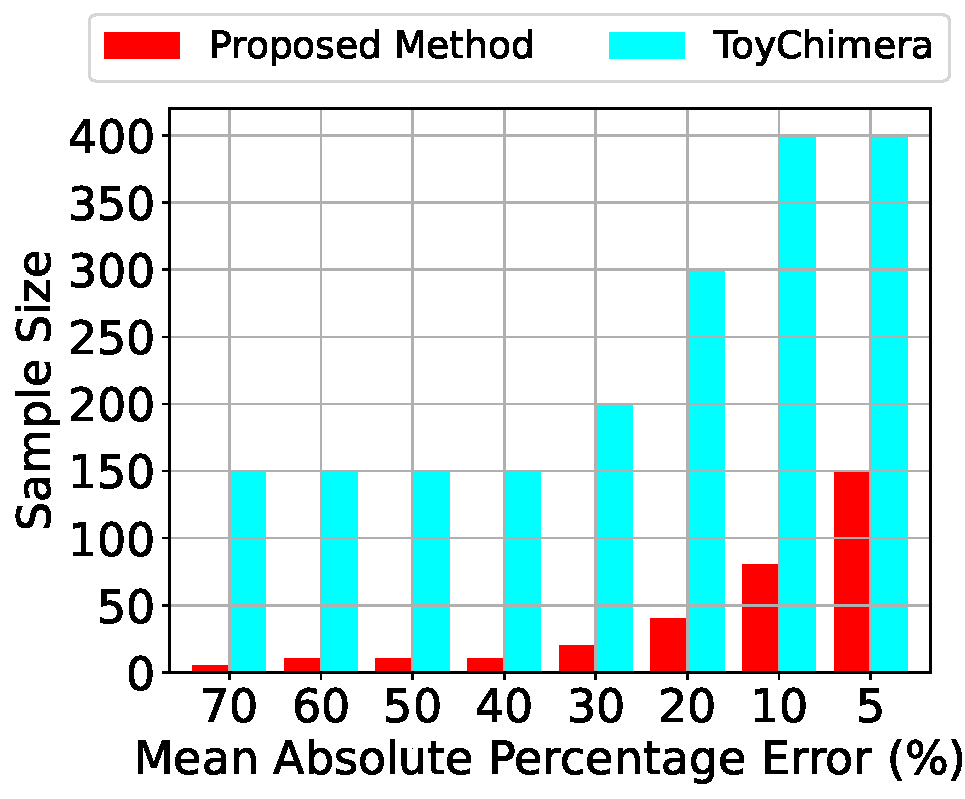
\includegraphics[width=.7\linewidth]{src/fig/toy_bar.pdf}
        \caption{\textbf{Performance prediction accuracy of ChimeraTL and ToyChimera}}
        \label{fig:toy}
    \end{minipage}
\end{figure*}

Fig.~\ref{fig:results} shows the performance prediction accuracy of the transfer learning methods.
The x-axis represents the number of samples from the target environment and the y-axis represents the mean absolute percentage error (MAPE)\cite{Valov, l2s, mape} of the performance prediction model.

While the existing methods do not show a large difference with 10 samples, ChimeraTL already separates itself from the other methods, reducing the prediction error to below 40\%.
This result demonstrates the effectiveness of ChimeraTL's linear transformation learning that aims to linearly transform and reuse the source data for the target model construction.
ChimeraTL further reduces the prediction error to under 10\% with 80 samples, while other methods require at least 150 samples to achieve the same accuracy.
ChimeraTL's steady improvement in prediction accuracy with increased number of samples justifies its strategy to prioritize sampling for non-linear parameters once enough samples are collected for the linear transformation learning.
With ChimeraTL achieving the best prediction accuracy for almost all the number of samples, it is clear that ChimeraTL can build an accurate performance prediction model with fewer samples from the target environment. 

Contrary to the findings of the previous work that ModelShift needs less than 10 samples to learn the linear transformation\cite{Valov}, ModelShift requires 80 samples to achieve its best prediction accuracy of just around 40\% in our experiments.
This is because there are non-linear parameters in LineairDB that interfere with the learning of the linear transformation.
DataReuseTL and L2S+DataReuseTL display steady improvement in prediction accuracy, but their prediction accuracy never reaches below 40\% even with all available samples from the target environment because there is a huge difference between the DBMS performance in the source and target environments.
Even though ChimeraTL linearly transforms the source data and reuses it for the target model construction, the effect of negative transfer is minimized because ChimeraTL excludes the source data of non-linear parameters in the process.

Contrasting with the methods that suffer from the negative transfer, L2S shows a steady improvement in prediction accuracy as the number of samples increases.
Still, L2S generally requires twice as many samples as ChimeraTL to achieve the same prediction accuracy.
Since L2S does not use the source environment data at all to train the model, it requires more samples from the target environment to build a model with the same accuracy as ChimeraTL.

\subsection{Importance of Parameter Separation}
To understand the effect of parameter separation, we compare ChimeraTL with ToyChimera, a variant of ChimeraTL that does not separate parameters.
Essentially, ToyChimera is the same as ChimeraTL except (1) it does not exclude the data of non-linear parameters from the linear transformation learning and the source data reuse, and (2) it samples data randomly instead of giving priority to certain parameters at different stages of the sampling process.
Fig.~\ref{fig:toy} shows the performance prediction accuracy of ChimeraTL and ToyChimera, in addition to the baseline method.
% \begin{figure}[t]
%     \centering
%     \centerline{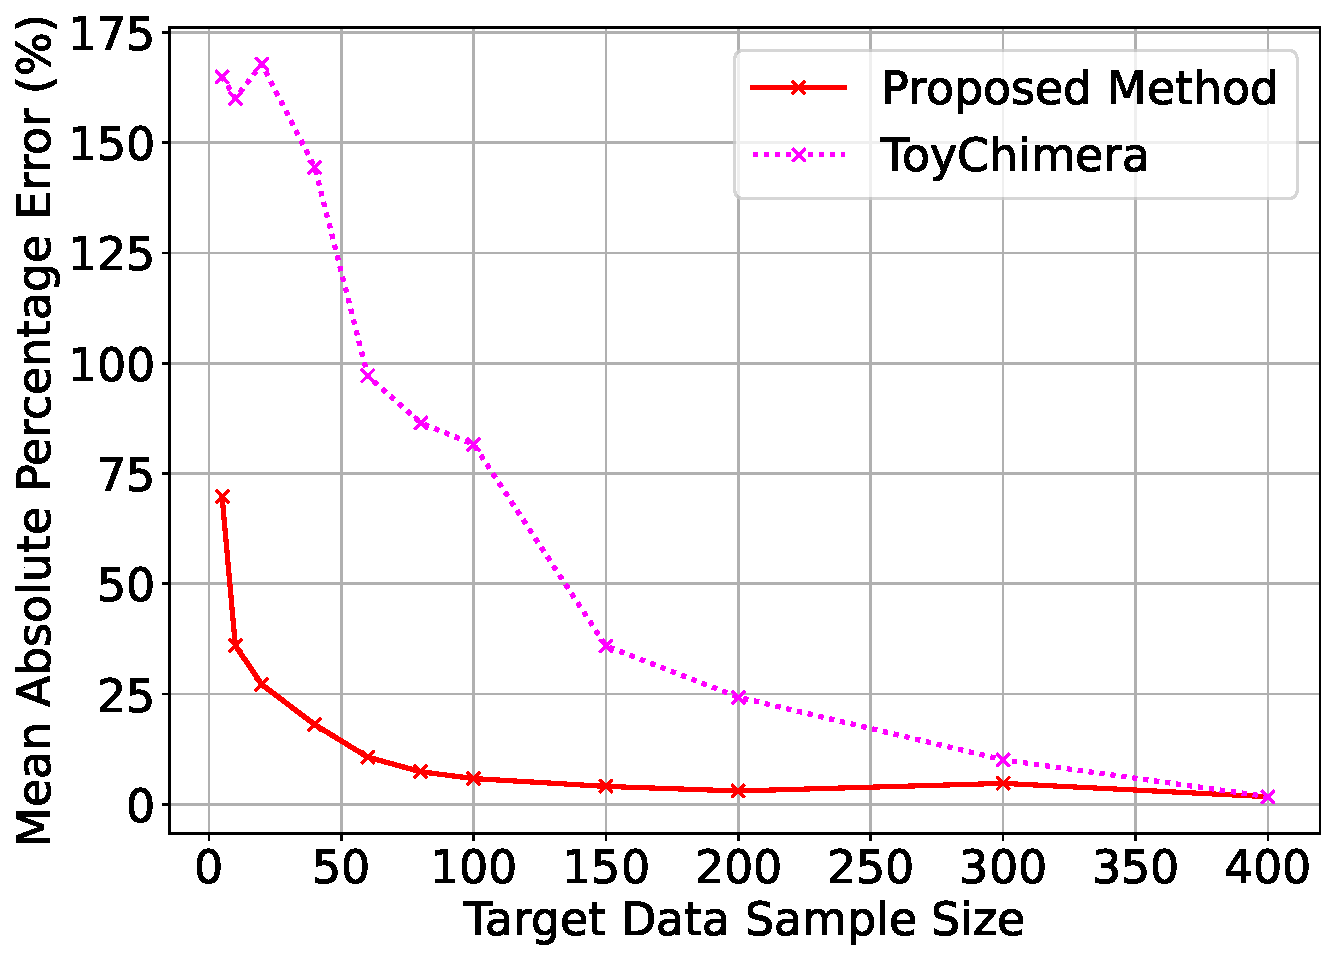
\includegraphics[width=0.475\textwidth]{src/fig/toy.pdf}}
%     \caption{\textbf{Performance prediction accuracy of ChimeraTL and ToyChimera}}
%     \label{fig:toy}
% \end{figure}

As shown in Fig.~\ref{fig:toy}, The prediction accuracy of ToyChimera significantly falls short when compared to that of ChimeraTL.
ToyChimera can only reduce the error to around 35\% with 150 samples, when ChimeraTL can reduce the error to below 5\% with the same number of samples.

As explained in Section~\ref{sec:eval:exst} and shown in Fig.~\ref{fig:results}, involving non-linear parameters in the linear transformation learning and reusing all the source data causes the negative transfer which significantly degrades the prediction accuracy.
ChimeraTL filters out the data of non-linear parameters for these processes so that it can reuse the source data without suffering from the negative transfer.
Consequently, ChimeraTL can build a more accurate performance prediction model with fewer samples from the target environment.
\section{Related Work}
In the field of DBMS, performance prediction models are commonly used to recommend optimal configurations for dynamic workloads using past data\cite{Ottertune,Onlinetune,cdbtune,mysql197}. 
Despite the common use of performance models in DBMS, few studies, like ResTune, leverage knowledge from different hardware environments to build a performance prediction model\cite{restune}.
ResTune used a meta-learning approach to combine models from multiple environments.
However, the main concern of performance prediction models in DBMS is not on the accuracy itself but on finding optimal configurations for a new workload.

On the other hand, several research efforts in the field of transfer learning have aimed to efficiently learn models on new hardware environments. These studies have shown that software performance on one hardware environment has a strong correlation with that on another environment\cite{Valov,jamshidi}. It has also been found that parameters that significantly impact performance are likely to be shared between the source and target environments\cite{jamshidi,l2s}. However, these studies were based on the results of configuring binary parameters, and it was unclear whether the results of these studies were applicable to DBMS, where many parameters have a wide range of values.

In this paper, we found that some parameters in DBMS are linear, but others are not.
This difference in parameters limited the performance of existing transfer learning techniques that assumed a strong linear relationship between the source and target environments\cite{Valov,datareuse}.
Therefore, we proposed a new transfer learning technique that can build an accurate performance model of DBMS with fewer samples by considering the characteristics of DBMS parameters.
\section{Conclusion}
We proposed a new transfer learning approach for building performance prediction models of DBMS.
Our proposed method is based on the observation that parameters can be divided into two groups: the parameters that have similar effects across different hardware environment and the parameters that do not.
We adopted a novel parameter separation technique which allowed us to employ different transfer learning methods for each group of parameters.
Our experimental results show that our proposed method requires less than half the amount of training data that the existing methods require to achieve the same prediction accuracy.

\section*{Acknowledgment}

The preferred spelling of the word ``acknowledgment'' in America is without 
an ``e'' after the ``g''. Avoid the stilted expression ``one of us (R. B. 
G.) thanks $\ldots$''. Instead, try ``R. B. G. thanks$\ldots$''. Put sponsor 
acknowledgments in the unnumbered footnote on the first page.

\bibliographystyle{IEEEtran}
\bibliography{src/refer}

% \vspace{12pt}
% \color{red}
% IEEE conference templates contain guidance text for composing and formatting conference papers. Please ensure that all template text is removed from your conference paper prior to submission to the conference. Failure to remove the template text from your paper may result in your paper not being published.

\end{document}
